%% Use the hmcposter class with the thesis document-class option.
\documentclass[thesis]{hmcposter}
\usepackage{graphicx}
\usepackage{natbib}
\usepackage{booktabs}
\usepackage{subfig}
\usepackage{amsmath}
\usepackage{textcomp}
\usepackage{url}
\usepackage{enumitem}
\setlist{leftmargin=2cm, labelsep=0.7cm}

%% Author of the thesis.
\author{Stetson Bost}

%% The year of your thesis poster's creation.
\posteryear{2017}

%% Thesis Title.
\title{Adaptive Nested Algorithms\\for Balanced Scheduling}

%% Advisor name.
\advisor{Weiqing Gu}

%% Define the \BibTeX command, used in our example document.
\providecommand{\bibtex}{{\rmfamily B\kern-.05em%
    \textsc{i\kern-.025em b}\kern-.08em%
    T\kern-.1667em\lower.7ex\hbox{E}\kern-.125emX}}


\pagestyle{fancy}

\begin{document}

\begin{poster}

\section{Introduction}
Scheduling is very important for staying organized and managing stress for both individuals and larger organizations.
With this project, we wanted to develop algorithms capable of creating effective, adaptable, and balanced schedules.

\section{Algorithm for Personal Scheduling}%
Our algorithm for creating personal schedules aims to accomplish all necessary tasks while maintaining a balanced schedule.
A schedule is a collection of relatively short \emph{time slots}, and contiguous time slots can form \emph{blocks}.
A group of consecutive blocks can form a \emph{section}, identified by it starting and ending blocks.
The algorithm has three nested steps.
\begin{enumerate}
	\item
		Assign tasks to sections.
	\item
		Assign tasks to blocks within sections. 
	\item
		Assign tasks to time slots within blocks.
\end{enumerate}
Each step takes into account various aspects of the tasks, including deadlines, estimated duration, and intensity. Additionally, each block has a minimum permissible amount of time reserved for non-work activities, which may or may not be structured, depending on user preference.
By maintaining near equal intensity levels among blocks, the algorithm prioritizes a balanced schedule.

\begin{figure}
  \centering
        \subfloat[][Start with a list of tasks that need to be completed.]{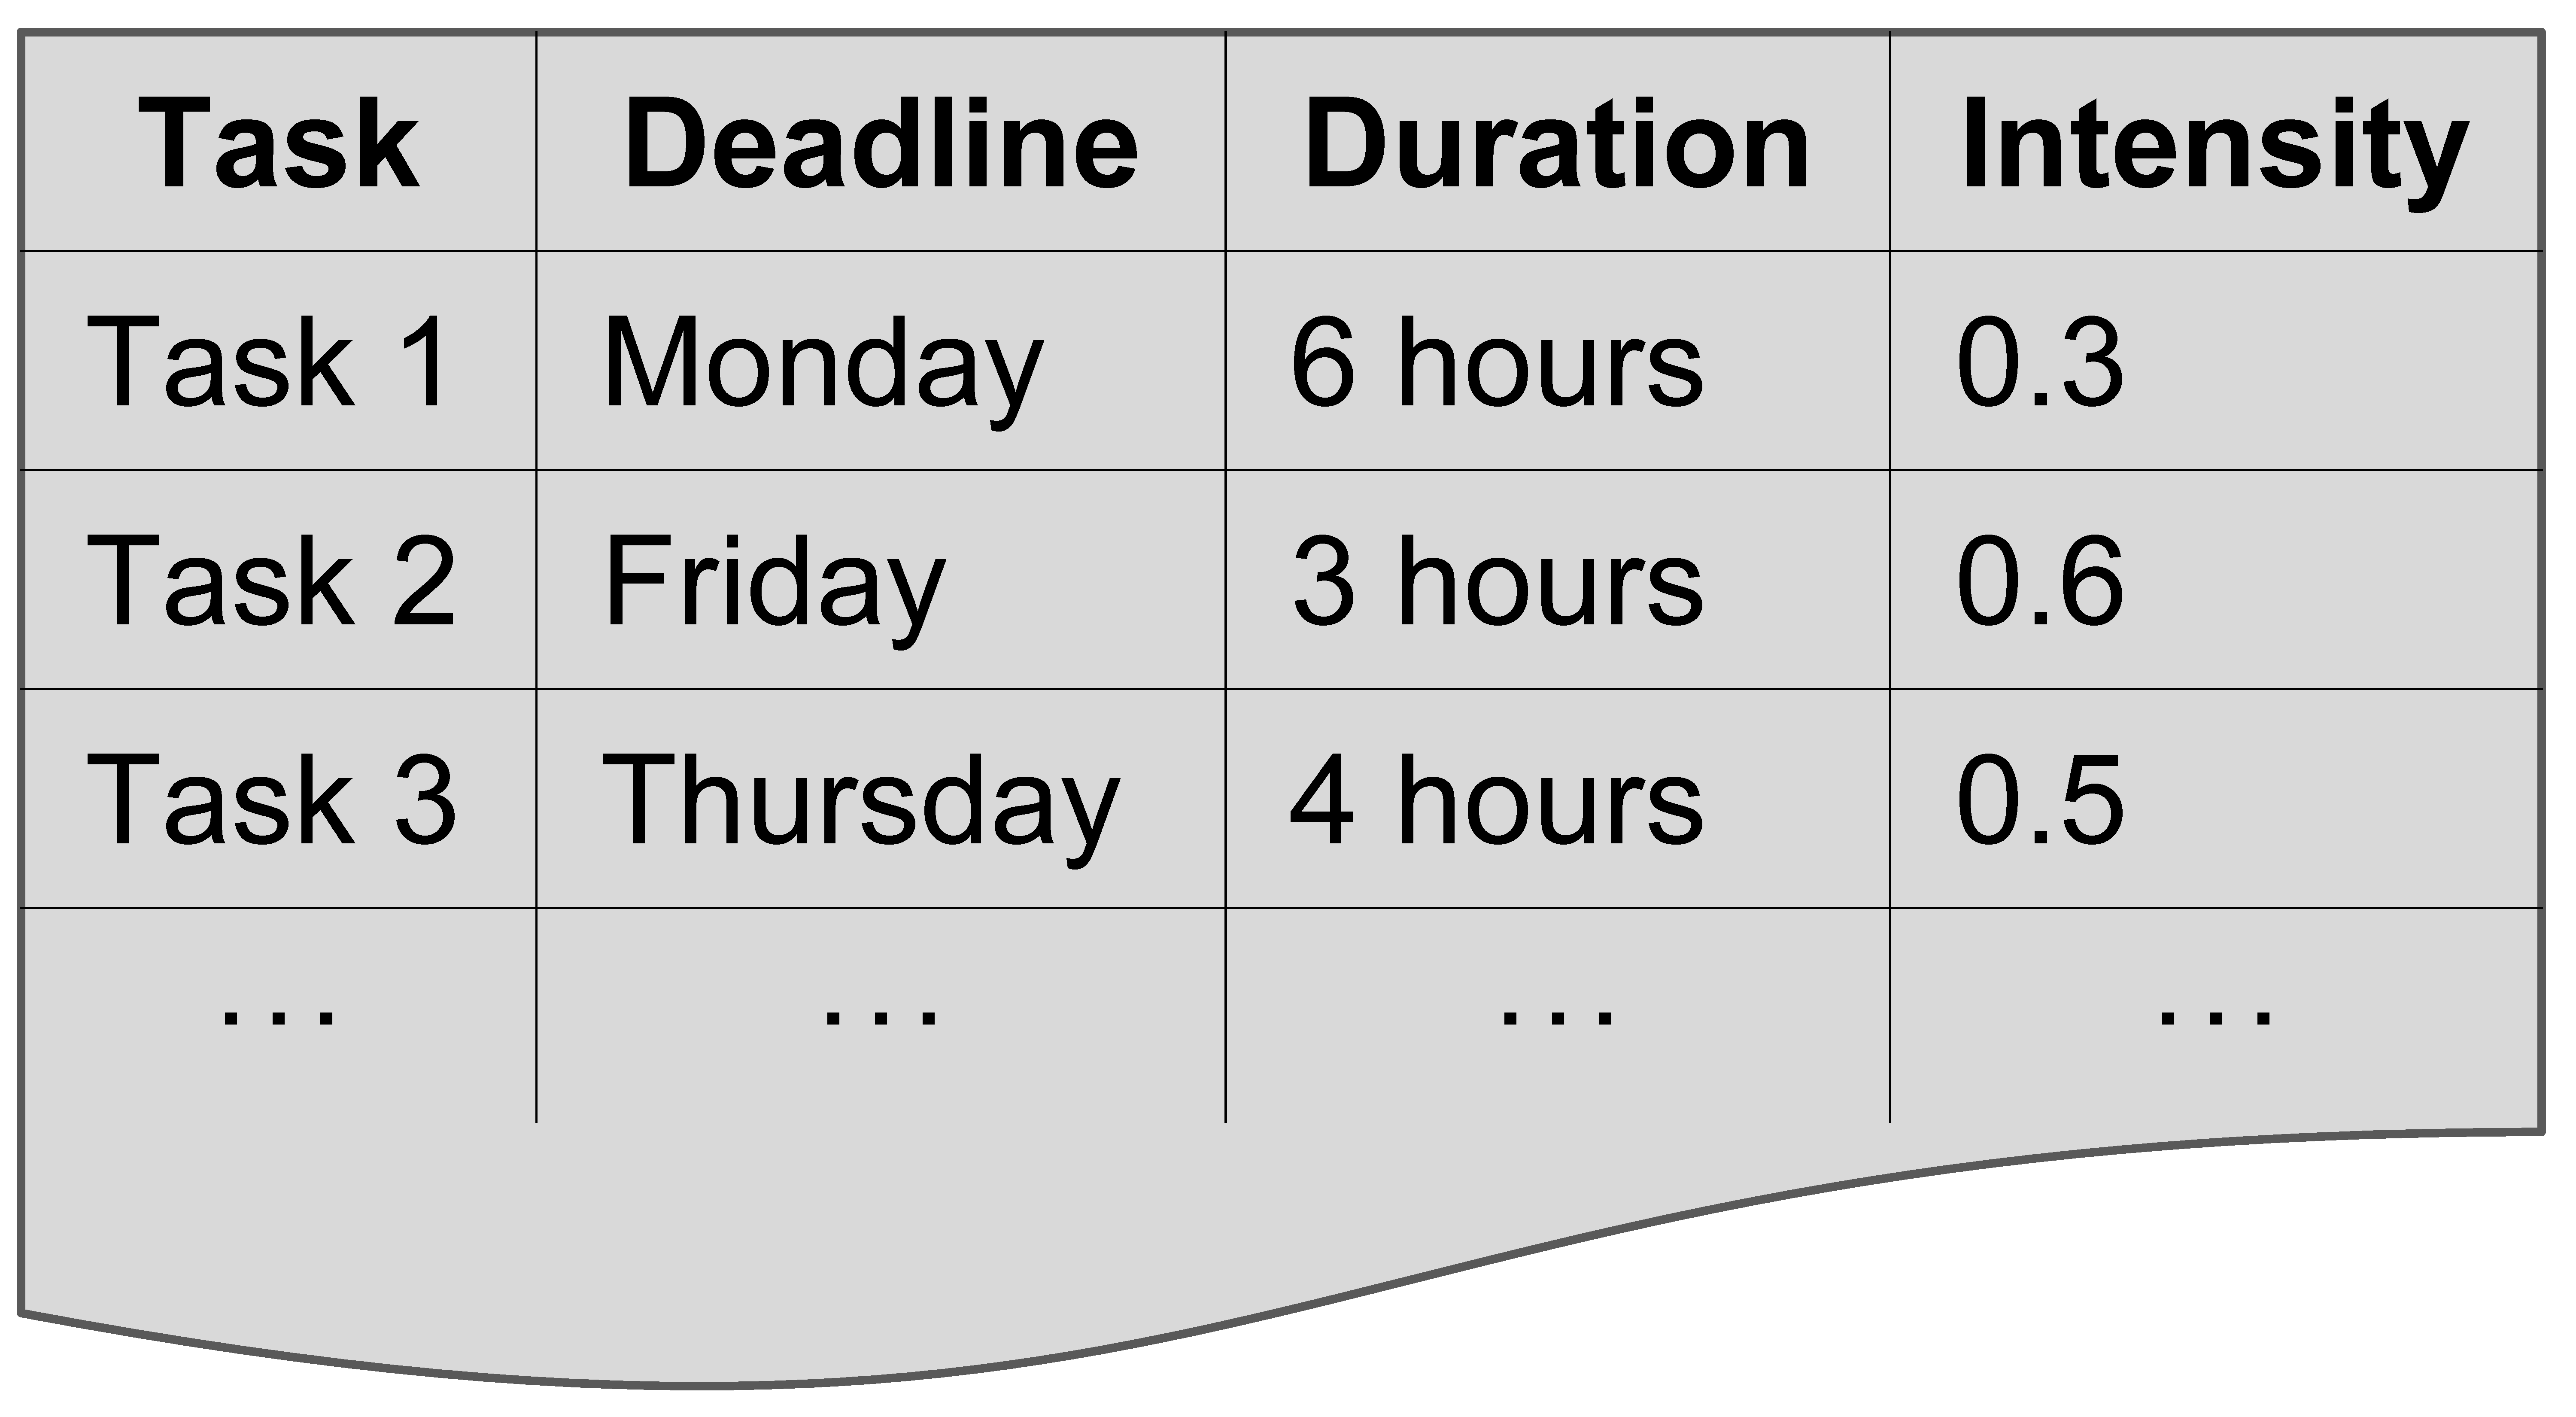
\includegraphics[scale=0.18]{TaskList.pdf}%
                \label{fig:small-mults-orig}%
        }\qquad\qquad
        \subfloat[][Step 1: Create a section made up of time blocks, and assign tasks to the section. Non-work time is treated as a task.]{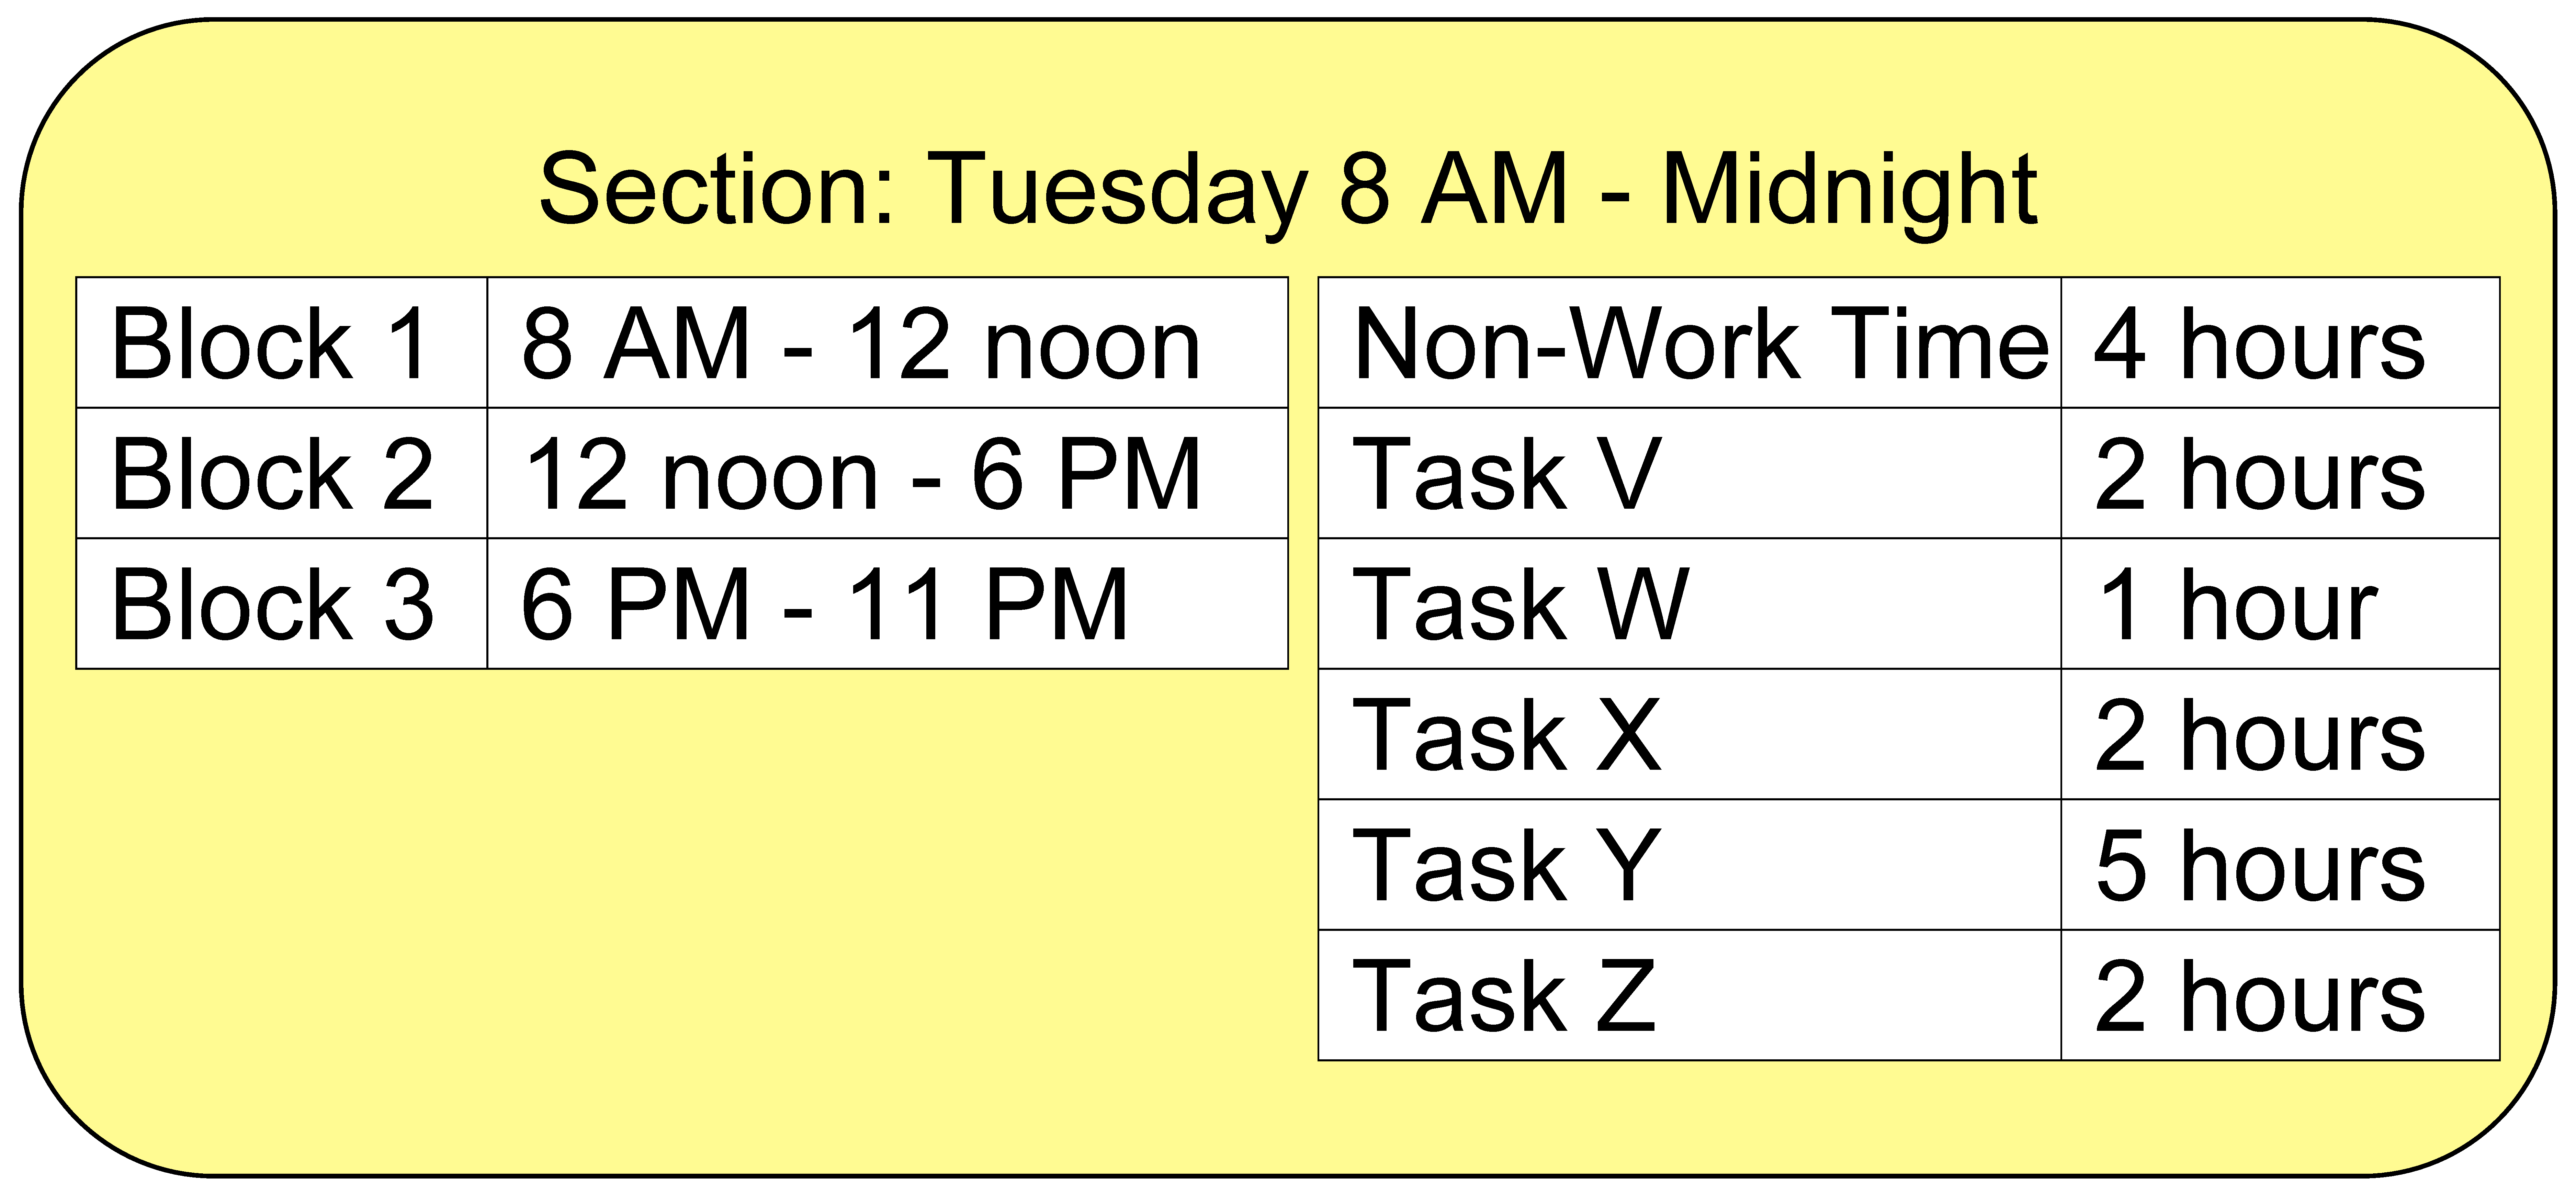
\includegraphics[scale=0.18]{Section.pdf}%
                \label{fig:small-mults-45}%
        }\\
        \subfloat[][Step 2: Assign tasks to each block in the section.]{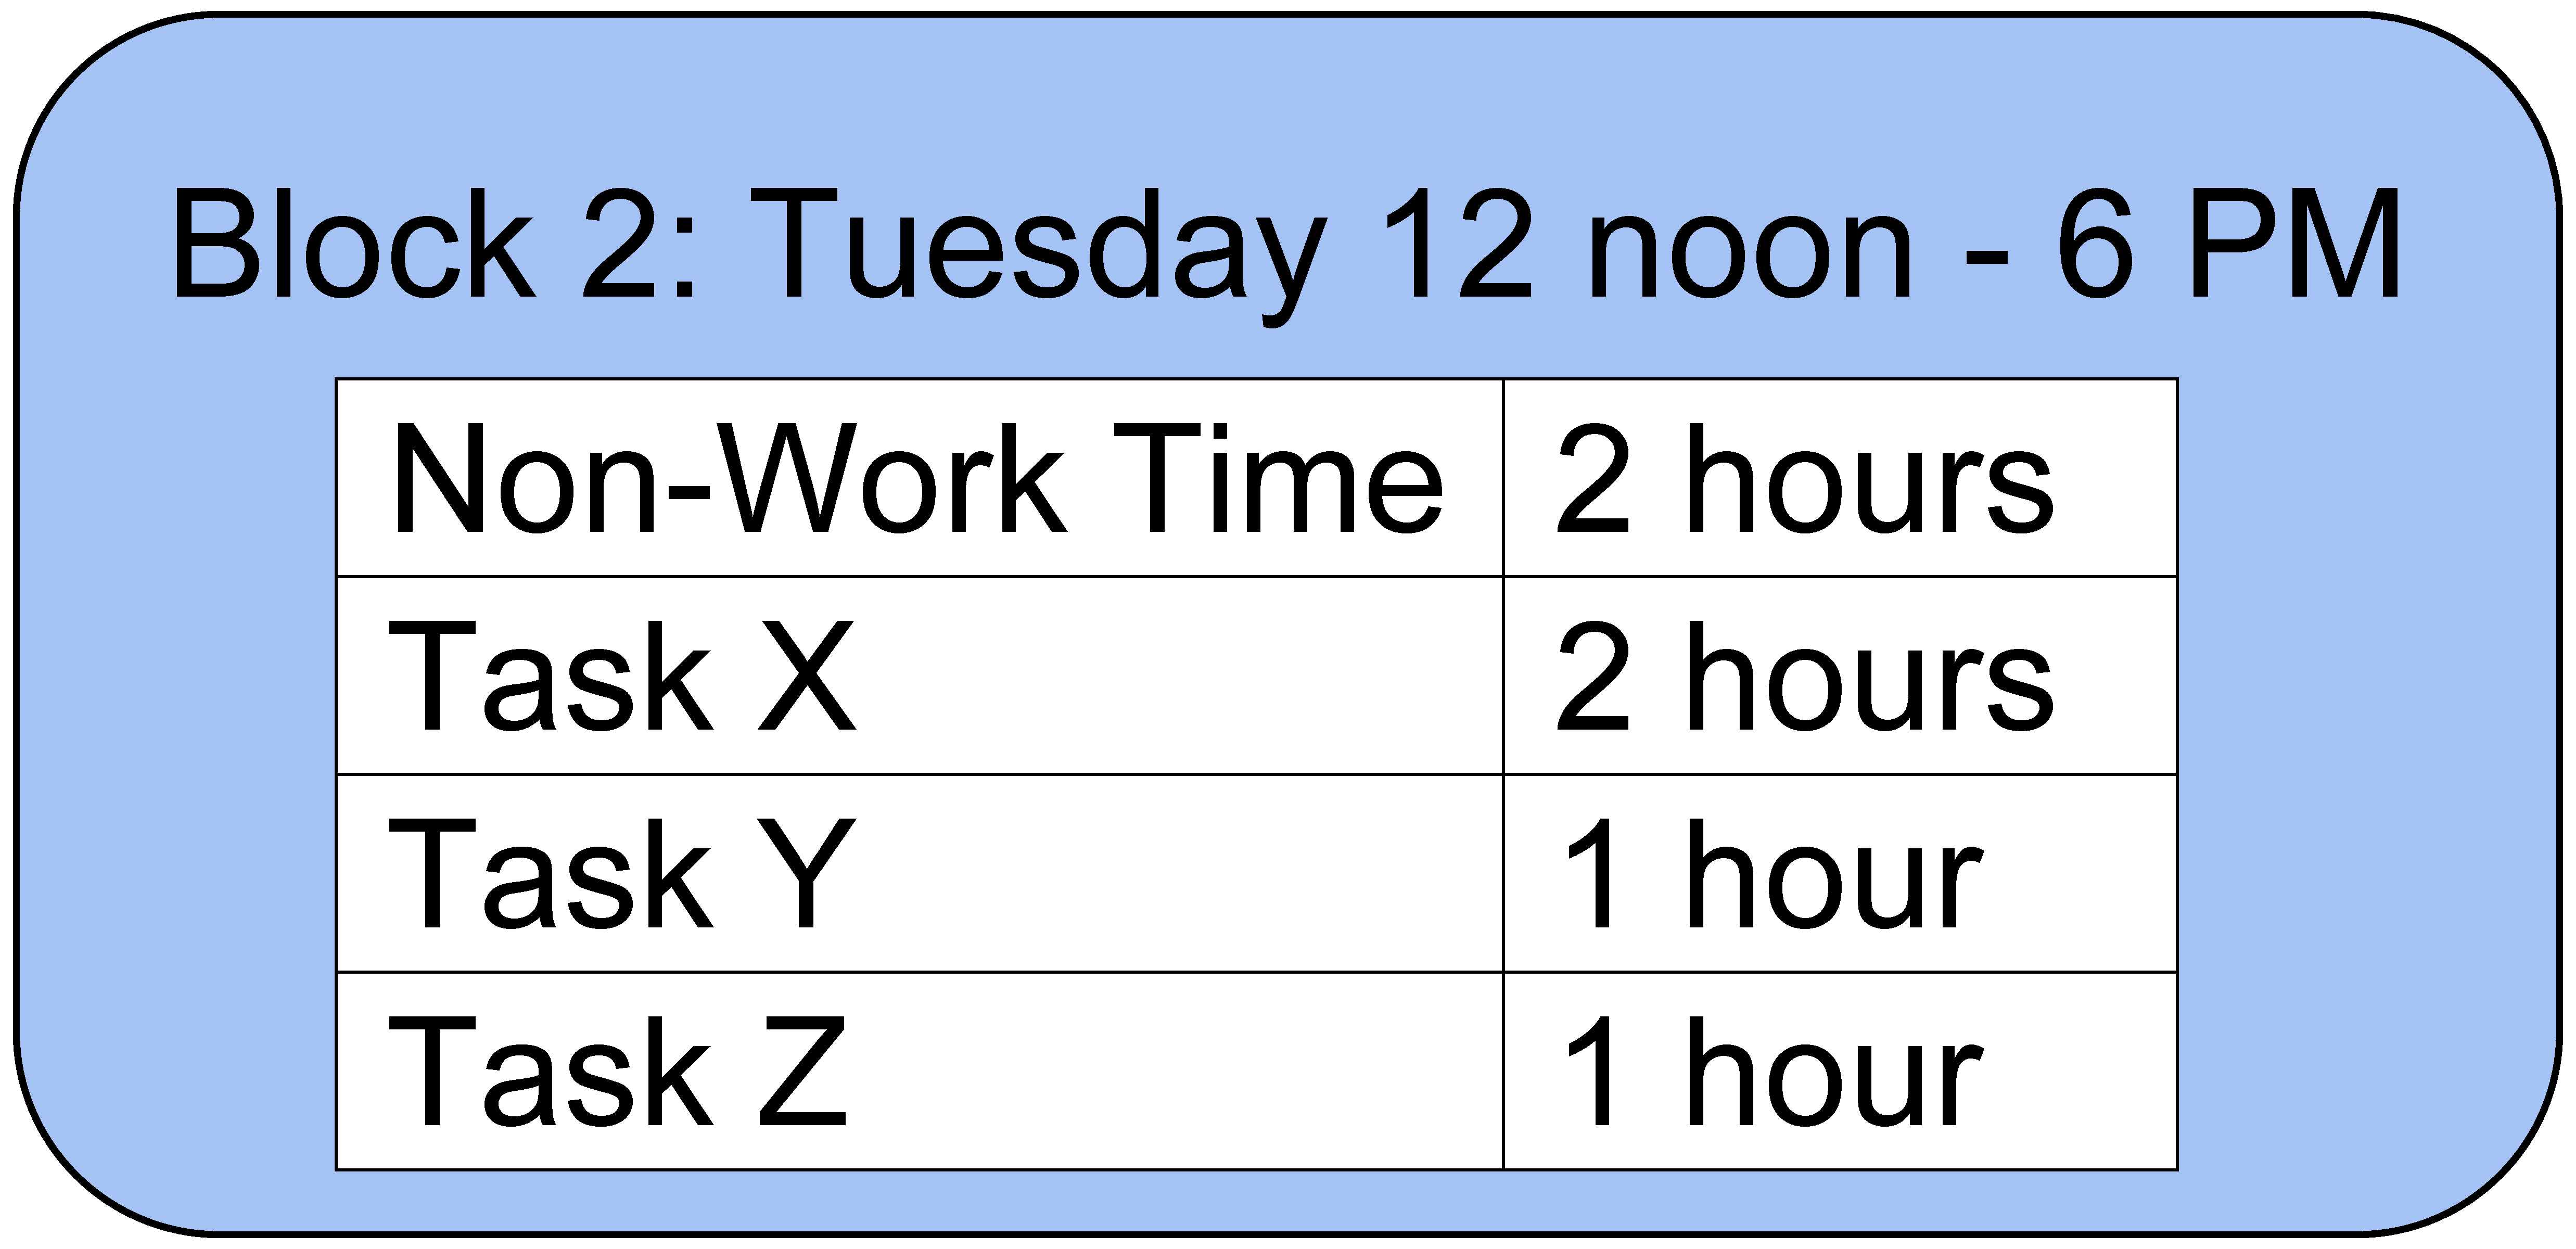
\includegraphics[scale=0.18]{Block.pdf}%
                \label{fig:small-mults-90}%
        }\qquad\qquad
        \subfloat[][Step 3: Schedule tasks within the block.]{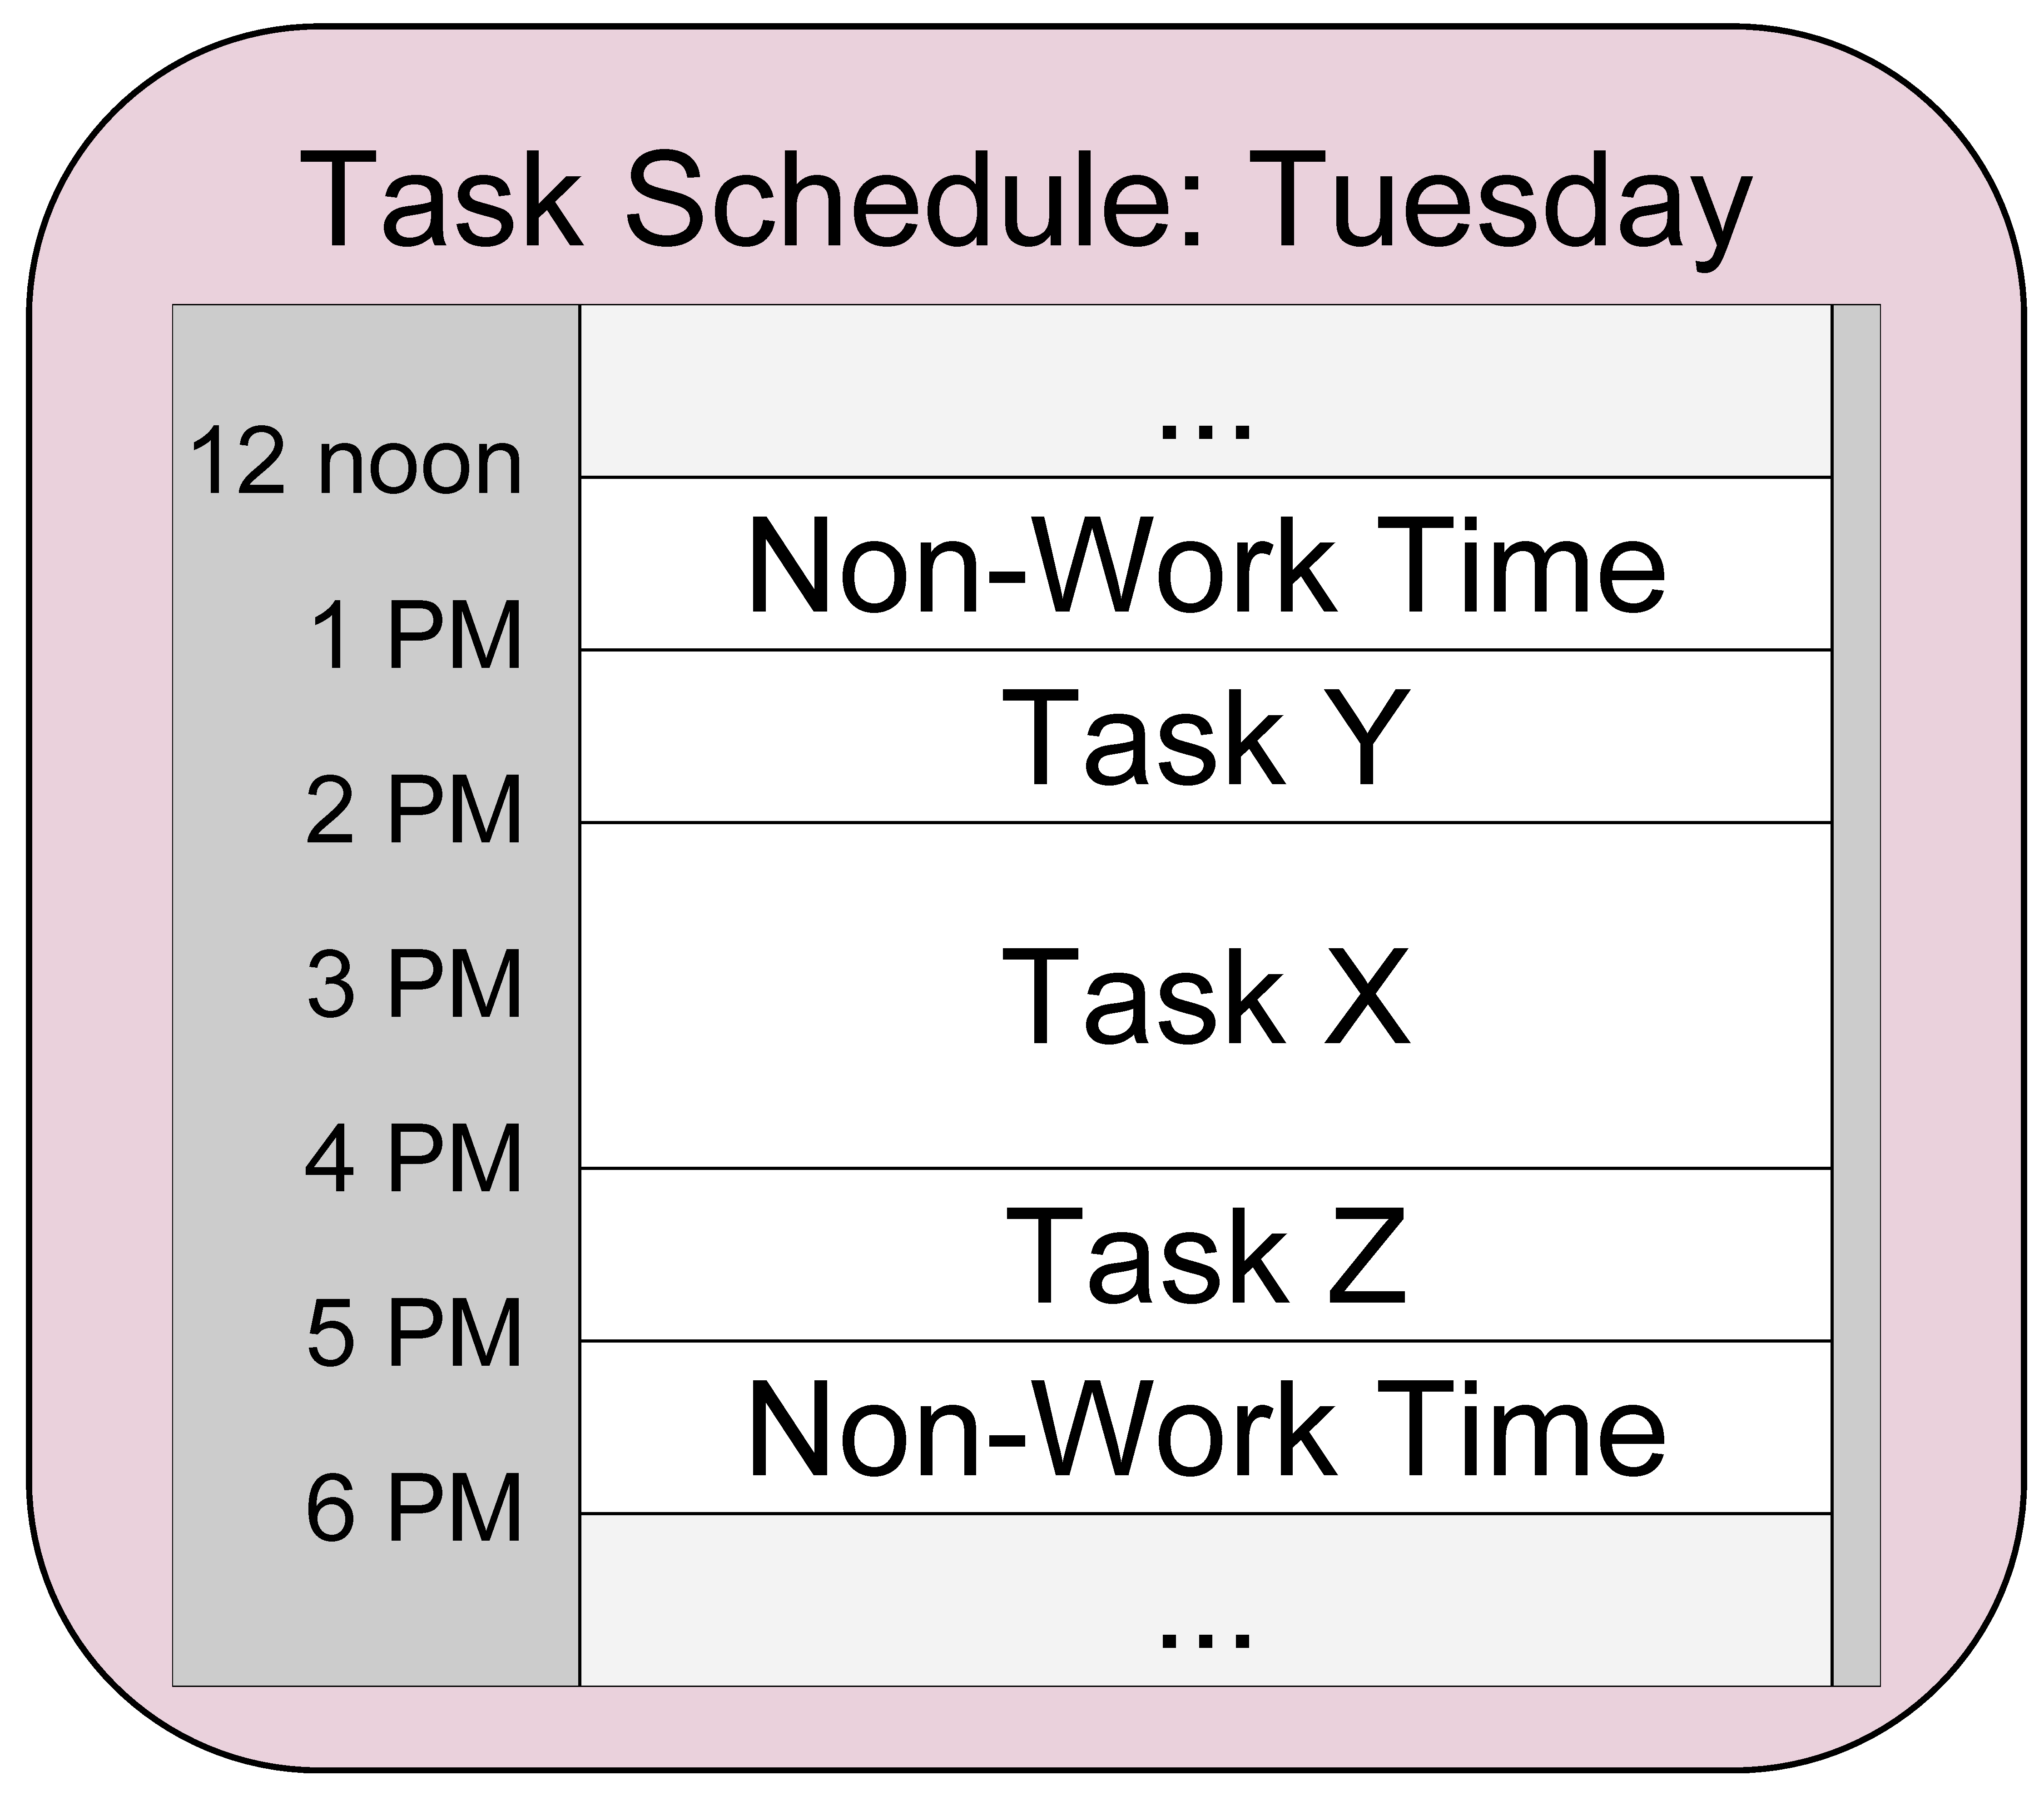
\includegraphics[scale=0.18]{Schedule.pdf}%
                \label{fig:small-mults-135}%
        }
  \caption[Small multiples]{Example for personal scheduling algorithm.}%
  \label{fig:small-multiples}
\end{figure}



\section{For Further Information}
For more information about this project, please contact \url{sbost@hmc.edu} or \url{gu@hmc.edu}.
%\columnbreak


\section{Algorithm for Event Scheduling}
Members of a group often have to schedule events where a number people must attend.
We wanted to create an algorithm capable of scheduling events with multiple attendees.
An event can be either recurring (``regular'') or non-recurring (``special''), will have restrictions on available times, and may have a list of desired or required attendees.

\subsection{Probabilistic Approach}
One approach is to use historic data and a probabilistic version of the $k$-nearest neighbors algorithm to determine the likelihoods that all potential attendees will attend a specific event scheduled at potential times (Holmes).
By summing these likelihoods across all attendees, we are able to get the expected value for the number of people at the event.

\subsection{Nested Approach}
An alternate approach makes use of the nested personal scheduling algorithm detailed to the left with some slight modifications.
The basic structure of time slots, blocks, and sections is still the same, but it may be less likely to have adjacent blocks or contiguous sections, depending on the group's scheduling practices.
We treat events as tasks with possible time windows, and use those to create sections.
In place of task intensity, we use a quantity that describes the priority of the event.
We also create some conditions for balance, such as demands on the frequency of regular and special events.


\section{Future Work}
A good next step for this work would be to use code implement the algorithms so that they can be tested on a group of people.
To further validate the algorithms, it will be useful to test the algorithms on actual scheduling problems.
Ideally this testing should be with people and groups that are willing to try the schedules produced by the algorithm.
Additionally, for an group that uses a common calendar application, it might be possible to integrate the event scheduling algorithms with the calendar to automatically schedule events.


\section{References}
\bibliographystyle{hmcmath}
%\bibliography{sampleposter}
C.~C.~Holmes and N.~M.~Adams, 2002. \emph{A probabilistic nearest neighbour method for statistical pattern recognition}. \url{http://hedibert.org/wp-content/uploads/2016/02/holmes-adams-2002.pdf}.


\section{Acknowledgments}
I would like to thank my advisor, Professor Weiqing Gu, for her guidance throughout this research.
I am also very grateful for the kindness and generosity of the Rose Hills Foundation through their Science and Engineering Summer Undergraduate Research Fellowship, which has made this project possible.


\end{poster}

\end{document}

 
